\documentclass{article}
\usepackage{graphicx}
\usepackage[utf8]{inputenc}
\usepackage[T1]{fontenc}
\usepackage{pgfplots}
\usepackage{pgfplotstable} 
\usepackage{titlesec}
\usepackage{lipsum}
\usepackage{authblk}
\usepackage{algorithm}
\usepackage{amsmath}
\usepackage[noend]{algpseudocode}
\usepackage {tikz}
\usetikzlibrary {positioning}

\titleformat{\chapter}[display]{\normalfont\bfseries}{}{0pt}{\Large}

\begin{document}

\title{Aprendizado de Máquina: Trabalho Prático 2 (Boosting)}
\author{João Mateus de Freitas Veneroso}
\affil{Departamento de Ciência da Computação da Universidade Federal de Minas Gerais}

\maketitle

\section{Introdução}

Este relatório descreve a implementação do trabalho prático 2 da disciplina Aprendizado de Máquina. 
O trabalho consistiu em implementar um algoritmo de Boosting e treiná-lo no \textit{dataset}
Tic-Tac-Toe, que consiste em todas as combinações de jogadas possíveis no Jogo-da-Velha. A
avaliação da eficácia do modelo foi feita por meio da análise do erro simples, utilizando a
metodologia de \textit{K-Fold Cross-Validation} com 5 partições.

\section{Modelo}

Os algoritmos de \textit{Boosting} consistem em um agrupamento de múltiplos \textit{weak learners},
cuja classificação individual é apenas levemente correlacionada com a verdadeira classificação, 
com o objetivo de construir um classificador mais robusto. Uma das vantagens do \textit{Boosting} é
prevenir o fenômeno de \textit{Overfitting} quando os \textit{weak learners} fazem previsões independentes.

O algoritmo de \textit{Boosting} implementado neste trabalho foi o \textit{AdaBoost}. Os \textit{weak learners} 
utilizados foram os \textit{Decision Stumps}, que consistem em árvores de decisão com apenas 1 nível.
Experimentos também foram feitos com \textit{weak learners} mais complexos, no entanto, o resultado
foi pior do que quando utilizados os \textit{Decision Stumps}.

O \textit{Ada Boost} consiste em um processo iterativo que atribui um peso $ \alpha_i $ para cada 
\textit{weak learner} e classifica o dado com base em uma função de classificação binária $ H(x) $,
cujo valor (-1 ou 1), representa a classe correspondente à entrada $ x $. A definição de $ H(x) $ é:

\[
H(x) = sign(\alpha_1h_1(x) + \alpha_2h_2(x) + ... + \alpha_nh_n(x))
\]

onde $ h_i $ representa a previsão individual do \textit{weak learner} $ i $. O processo de treinamento 
do nosso algoritmo consiste em ajustar os valores $ \alpha_t $ para 
diminuir o erro empírico de $ H(x) $. À medida que cresce o número $ n $ de classificadores fracos,
o erro empírico tende a diminuir, convergindo para zero no limite da capacidade do modelo. À
cada iteração $ t $, selecionamos o classificador fraco com o menor erro empírico e 
calculamos o seu peso $ \alpha_t $ por meio da seguinte expressão:

\[
\alpha_t = \frac{1}{2} ln\left(\frac{1 - \epsilon_t}{\epsilon_t}\right)
\]

onde $ \epsilon_t $ é o erro empírico do classificador selecionado. No entanto, o erro empírico não
consiste apenas na classificação e avaliação simples do \textit{dataset} $ M $. Cada caso de treino 
$ x_i $ contribui com um peso $ w_i $ ao erro empírico $ \epsilon_t $, de forma que:

\[
\epsilon_t = \sum_{i \in M} w_{i,t} E(x_i)
\]

onde $ E(x_i) $ é uma função indicadora do erro no caso de treino $ i $. O cálculo de $ w_{i,t} $ se dá pela expressão:

\[
w_{i,t+1} = \frac{w_{i,t}}{z} e^{-\alpha_t h_t(x) y(x)}
\]

Finalmente, o processo pode ser repetido $ n $ vezes, adicionando um novo classificador a cada iteração
para que, assintoticamente, o erro empírico tenda à zero. Contudo, apesar do erro empírico tender à
zero, o erro ponderado individual do classificador adicionado tende a crescer a cada iteração. Pois,
à medida que prosseguimos com o treinamento, o peso dos casos mais difíceis tende a aumentar
e os padrões se tornam cada vez mais complicados de discernir, de forma que, no limite,
os novos classificadores passam a errar aproximadamente 50\% das vezes.

\subsection{Classificadores Fracos}

Os classificadores fracos são calculados por meio do algoritmo de construção de árvores 
binárias de decisão CART. O CART utiliza uma estratégia de particionamento do espaço de decisão 
gulosa, na qual os cortes são escolhidos por meio da minimização de uma função de perda. O
nosso modelo utiliza o índice de impureza de Gini para determinar a ordem dos cortes. Ele representa
uma medida da probabilidade de atribuir um rótulo errado aos dados em um processo estocástico e
ele pode ser calculado pela expressão:

\[
G = \sum_{i = 1}^{J} f_i (1 - f_i) = \sum_{i = 1}^{J} f_i - f_i^2
\]

onde $ J $ é o número de classes e $ f_i $ é a frequência da classe $ i $ na partição. Observe que
$ \sum_{i = 1}^{J} f_i = 1 $, pois a soma da frequência de todas as classes na partição tem de
ser o total da partição. Assim:

\[
G = 1 - \sum_{i = 1}^{J} f_i^2
\]

Como explicado anteriormente, um peso $ w_j $ é atribuído a cada ponto do espaço amostral. Dessa
forma, para calcular a frequência $ f_i $ da classe $ i $ na partição, utilizamos a seguinte expressão:

\[
f_i = \frac{\sum_{j : y(j) = i} w_j}{\sum_{j} w_j}
\]

onde $ j $ são pontos dentro da partição e $ y(j) $ é a classe à qual aquele ponto pertence. Portanto,
a frequência $ f_i $ é simplesmente o peso dos pontos que pertencem à classe $ i $ dividida pela soma
dos pesos de todos os pontos na partição.

Finalmente, a cada iteração do algoritmo, o corte com a menor impureza de Gini é escolhido até que 
a árvore atinja o tamanho máximo ou as classes estejam perfeitamente separadas, o que corresponde a 
um índice de Gini igual à zero. No caso específico dos \textit{Decision Stumps}, apenas um corte 
é realizado.

\subsection{Cross-Validation}

O \textit{dataset} utilizado nos experimentos possui 958 exemplos de configurações de tabuleiros
do Jogo-da-Velha com o resultado positivo se o jogador "X" ganhou o jogo ou negativo, caso contrário. 
Para avaliar a eficácia dos modelos utilizamos a metodologia de \textit{K-Fold Cross-Validation} com 5 \textit{folds}. 
Primeiramente, os dados foram embaralhados de forma aleatória e divididos em cinco \textit{folds} com: 191, 191, 
191, 191 e 193 exemplos. Para cada número $ m $ de iterações do \textit{Ada Boost}, o modelo foi
treinado com 4 partições e o erro de teste foi calculado na partição excluída. O processo
foi repetido com as 5 combinações possíveis (cada vez excluindo uma das partições do conjunto de treinamento).
O erro para aquele número de iterações $ m $ foi calculado por meio da média simples 
dos valores obtidos em cada uma das combinações.

\section{Experimentos}

\begin{figure}
  \center
  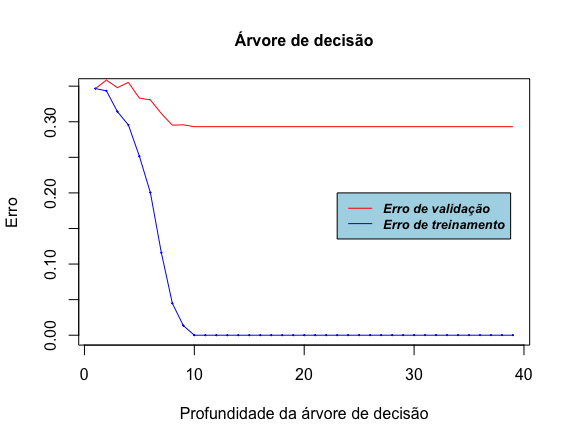
\includegraphics[width=256px]{decision_tree.png}
  \caption{Árvore de decisão}
  \label{fig:decision_tree}
\end{figure}

Três experimentos foram feitos no \textit{dataset} Tic-Tac-Toe. O primeiro
experimento mediu o erro de treinamento e o erro de validação para o algoritmo de árvore de decisão
CART descrito na seção anterior, conforme a altura máxima da árvore variava de 1 a 40 nós. O
resultado está descrito na figura \ref{fig:decision_tree}. A árvore de decisão é muito eficiente no
sentido de reduzir o erro de treinamento, alcançando erro zero com uma profundidade de apenas 10
nós. No entanto, por meio de \textit{Cross Validation} é possível
perceber que esta eficiência não se traduz para os exemplos fora dos casos de treino. 
Isso acontece por conta do \textit{overfitting}. No caso particular deste \textit{dataset}, aproximadamente
65\% dos casos tem a saída "positivo", portanto, na ausência de treinamento é possível obter uma
taxa de erro de aproximadamente 35\% meramente atribuindo o valor positivo à todos os casos. Logo,
podemos perceber que a árvore de decisão não consegue obter um ganho de performance muito grande em
relação à previsão sem treinamento.

\begin{figure}
  \center
  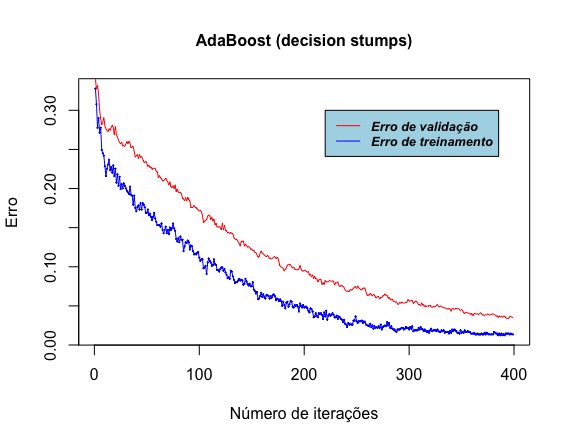
\includegraphics[width=256px]{adaboost.png}
  \caption{AdaBoost (decision stumps)}
  \label{fig:adaboost}
\end{figure}

O segundo experimento consistiu em mensurar o erro de treinamento e o erro de validação de 1 a 400 iterações do \textit{Ada Boost}
utilizando \textit{Decision Stumps} como \textit{weak learners}. A figura \ref{fig:adaboost} mostra o resultado do experimento.
Diferente da árvore de decisão, o AdaBoost reduz consideravelmente o erro de validação, o que garante que o resultado do algoritmo
vai se traduzir em um bom desempenho fora dos casos de treinamento. Também é possível notar que a convergência do erro de treinamento
é mais lenta.

\begin{figure}
  \center
  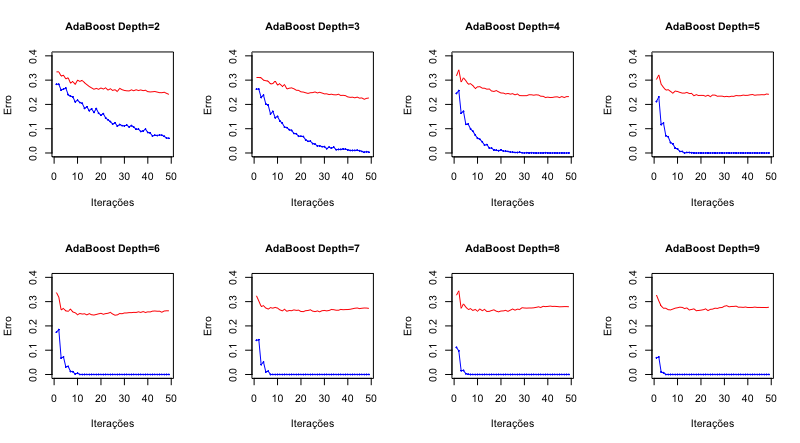
\includegraphics[width=360px]{adaboost_varying_depths.png}
  \caption{AdaBoost com modelos complexos}
  \label{fig:adaboost_depth}
\end{figure}

O terceiro experimento consistiu em variar a complexidade dos \textit{weak learners} para averiguar o
fenômeno de \textit{Overfitting} quando o AdaBoost utiliza modelos mais complexos. Para isso,
foram construídos 8 modelos diferentes, onde a altura das árvores de decisão variou de 2 a 9 nós. O resultado do experimento está 
descrito na figura \ref{fig:adaboost_depth}. Os resultados são significativamente piores do que no caso dos \textit{Decision Stumps},
os algoritmos ficaram limitados à 50 iterações porque o erro de validação não varia muito a partir disso e mais iterações prejudicariam 
a visualização dos gráficos. É possível perceber que, quanto maior é a complexidade dos \textit{weak learners}, mais rápido o erro
de treinamento converge para zero, no entanto, pior é a convergência do erro de validação. Como no caso da árvore de decisão sozinha,
isso acontece devido ao \textit{Overfitting}. E, com isso concluímos que o \textit{AdaBoost} é mais eficiente com modelos 
muito simples.

\section{Conclusão}

Este relatório descreveu a implementação do algoritmo \textit{Ada Boost} de acordo com a definição do 
trabalho prático 2 da disciplina Aprendizado de Máquina. A partir dos experimentos, concluímos que o 
\textit{AdaBoost} com \textit{Decision Stumps} é um modelo eficiente que alcança bons resultados
fora dos exemplos de treinamento.

\end{document}
\grid
